\documentclass[tikz,border=6pt]{standalone}
\usepackage{tikz}
\usetikzlibrary{arrows.meta,angles,quotes}
\definecolor{nebula}{HTML}{6366F1}
\definecolor{spark}{HTML}{14B8A6}
\definecolor{ink}{HTML}{334155}
\begin{document}
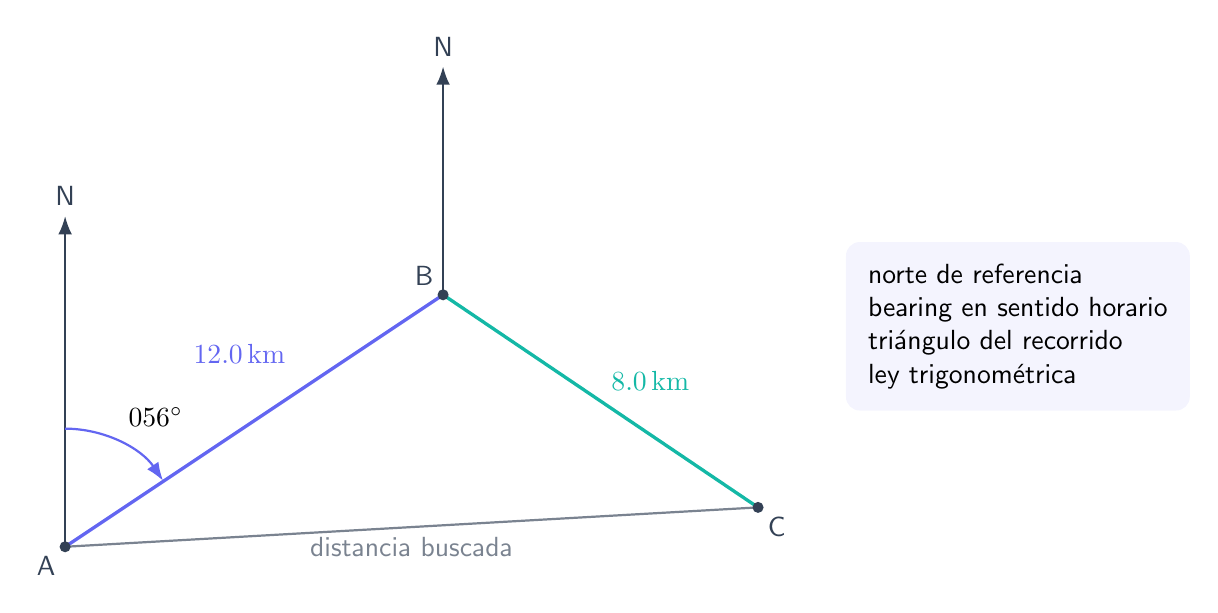
\begin{tikzpicture}[font=\sffamily,>=Latex]
  \coordinate (A) at (0,0); \coordinate (B) at (4.8,3.2); \coordinate (C) at (8.8,0.5);
  \draw[very thick,nebula] (A)--(B) node[pos=0.64,above left=4pt] {$12.0\,\mathrm{km}$};
  \draw[very thick,spark] (B)--(C) node[midway,above right] {$8.0\,\mathrm{km}$};
  \draw[thick,ink!65] (A)--(C) node[midway,below] {distancia buscada};
  \draw[->,thick,ink] (A)--(0,4.2) node[above] {N};
  \draw[->,thick,ink] (B)--(4.8,6.1) node[above] {N};
  \draw[->,nebula,thick] (0,1.5) arc[start angle=90,end angle=34,radius=1.5];
  \node[fill=white] at (1.15,1.65) {$056^\circ$};
  \fill[ink] (A) circle(2pt) node[below left] {A};
  \fill[ink] (B) circle(2pt) node[above left] {B};
  \fill[ink] (C) circle(2pt) node[below right] {C};
  \node[align=left,fill=nebula!7,rounded corners=5pt,inner sep=8pt] at (12.1,2.8) {norte de referencia\\bearing en sentido horario\\tri\'angulo del recorrido\\ley trigonom\'etrica};
\end{tikzpicture}
\end{document}
